\documentclass[11pt,psfig]{article}
\usepackage{epsfig}
\usepackage{times}
\usepackage{amssymb}
\usepackage{float}

\newcount\refno\refno=1
\def\ref{\the\refno \global\advance\refno by 1}
\def\ux{\underline{x}}
\def\uw{\underline{w}}
\def\bw{\underline{w}}
\def\ut{\underline{\theta}}
\def\umu{\underline{\mu}} 
\def\bmu{\underline{\mu}} 
\def\be{p_e^*}
\newcount\eqnumber\eqnumber=1
\def\eq{\the \eqnumber \global\advance\eqnumber by 1}
\def\eqs{\eq}
\def\eqn{\eqno(\eq)}

 \pagestyle{empty}
\def\baselinestretch{1.1}
\topmargin1in \headsep0.3in
\topmargin0in \oddsidemargin0in \textwidth6.5in \textheight8.5in
\begin{document}
\setlength{\parskip}{1.2ex plus0.3ex minus 0.3ex}


\thispagestyle{empty} \pagestyle{myheadings} \markright{Homework
6: CS 274A, Probabilistic Learning: Winter 2014}



\title{CS 274A Homework 6}
\author{Probabilistic Learning: Theory and Algorithms, CS 274A, Winter 2014}
\date{Due Date: Wednesday March 12th in class}

\maketitle

\vfill\eject

\subsection*{Solution to Problem 1, Part 1}

Using Bayes rule we need to compute the following
\[
p(c_1|x) = \frac{p(x|c_1)p(c_1)}{p(x|c_1)p(c_1) + p(x|c_2)p(c_2)}
\]
Find when that is equal to 0.5 as that is the decision boundary. This occurs when
\[
\frac{1}{2} = \frac{1}{1 + \frac{p(x|c_2)p(c_2)}{p(x|c_1)p(c_1)}}
\]
It thus occurs when
\[
\frac{p(x|c_2)p(c_2)}{p(x|c_1)p(c_1)} = 1
\]
This is the same as
\[
\frac{p(x|c_2)}{p(x|c_1)} = \frac{p(c_1)}{p(c_2)}
\]
Let
\[
K_1 = \frac{1}{\sigma_1 \sqrt{2\pi}}
\]
\[
K_2 = \frac{1}{\sigma_2 \sqrt{2\pi}}
\]
\[
f_1(x) = \frac{(x-\mu_1)^2}{\sigma_1^2}
\]
\[
f_2(x) = \frac{(x-\mu_2)^2}{\sigma_2^2}
\]
We now have to solve the following
\[
\frac{K_2 \cdot e^{-f_2(x)/2}}{K_1 \cdot e^{-f_1(x)/2}} = \frac{p(c_1)}{p(c_2)}
\]
Let
\[
Q = \frac{p(c_1)K_1}{p(c_2)K_2} = \frac{p(c_1)\sigma_2}{p(c_2)\sigma_1}
\]
Then we have to solve the following
\[
\frac{e^{-f_2(x)/2}}{e^{-f_1(x)/2}} = Q
\]
\[
e^{f_1(x) - f_2(x)} = Q^2
\]
\[
f_1(x) - f_2(x) = 2 log(Q)
\]
\[
\frac{(x-\mu_1)^2}{\sigma_1^2} - \frac{(x-\mu_2)^2}{\sigma_2^2} = 2 log(Q)
\]
Let $S = 2 log(Q) \sigma_2^2 \sigma_1^2$ then it holds that
\[
\sigma_2^2(x-\mu_1)^2 - \sigma_1^2(x-\mu_2)^2 = S
\]
Expanding and then collecting terms together we get
\[
x^2(\sigma_1^2 - \sigma_2^2) + 2x(\mu_1 \sigma_2^2 - \mu_2 \sigma_1^2) + (\sigma_1^2 \mu_2^2 - \sigma_2^2 \mu_1^2 - S) = 0
\]
We now let
\[
a = \sigma_2^2 - \sigma_1^2
\]
\[
b = 2(\mu_2 \sigma_1^2 - \mu_1 \sigma_2^2)
\]
\[
c = \sigma_2^2 \mu_1^2 - \sigma_1^2 \mu_2^2 - S
\]
Then the solutions are the roots of the quadratic equation $ax^2 + bx + c = 0$ which are as follows
\[
x = \frac{-b \pm \sqrt{b^2 - 4ac}}{2a}
\]

\subsection*{Solution to Problem 1, Part 2}

For this problem we will be using
\[
p(x|c_1) = \frac{1}{\sqrt{2\pi}} e^{- \frac{x^2}{2}}
\]
\[
p(x|c_2) = \frac{1}{\sqrt{6\pi}} e^{- \frac{(x-3)^2}{6}}
\]
To get the decision boundaries we will solve the quadratic equation with
\[
a = 2
\]
\[
b = 6
\]
\[
Q = \sqrt{3}
\]
\[
S = 2 log(Q) 3 = 3log(3)
\]
\[
c = -9 - 3 log(3)
\]
After putting this all into Matlab, we end up with the following plot
\begin{figure}[H]
\centering
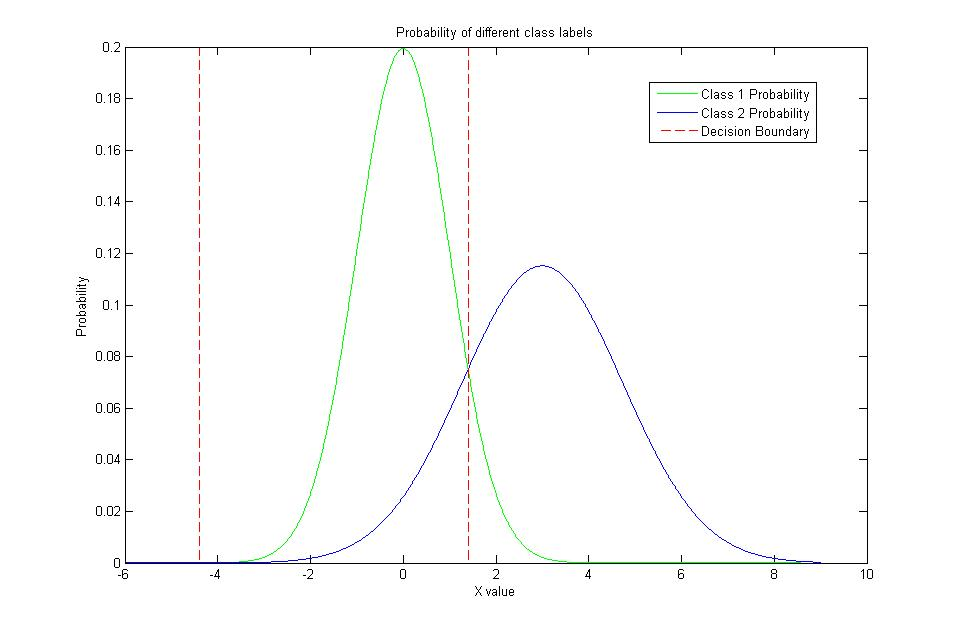
\includegraphics[height=5in]{prob1plot.jpg}
\caption{Probability of Class Labels with decision boundaries marked}
\end{figure}

\subsection*{Solution to Problem 1, Part 3}

For this case, if we let a and b be the decision boundaries and E be the error, then
\[
E = \int_{-\infty}^{a}{p(c_1|x)p(x) \, dx} + \int_{a}^{b}{p(c_2|x)p(x) \, dx} + \int_{a}^{\infty}{p(c_1|x)p(x) \, dx}
\]
For our case we can simplify this to
\[
E = \int_{-\infty}^{a}{p(x|c_1)p(c_1) \, dx} + \int_{a}^{b}{p(x|c_2)p(c_2) \, dx} + \int_{a}^{\infty}{p(x|c_1)p(c_1) \, dx}
\]
\[
E = 0.5(\int_{-\infty}^{a}{p(x|c_1) \, dx} + \int_{a}^{b}{p(x|c_2) \, dx} + \int_{a}^{\infty}{p(x|c_1) \, dx})
\]
For this case, according to the Matlab computation, we have $a=-4.3979$ and $b=1.3979$. \\
According to Wolfram Alpha
\[
\int_{-\infty}^{a}{p(x|c_1) \, dx} = \frac{1}{\sqrt{2\pi}} \int_{-\infty}^{-4.3979}{e^{-x^2/2} \, dx} = \frac{0.0000136991}{\sqrt{2\pi}} = 5.46515 \cdot 10^{-6}
\]
\[
\int_{a}^{b}{p(x|c_2) \, dx} = \frac{1}{\sqrt{6\pi}} \int_{-4.3979}^{1.3979}{e^{-(x-3)^2/6} \, dx} = \frac{0.77055}{\sqrt{6\pi}} = 0.177480
\]
\[
\int_{b}^{\infty}{p(x|c_1) \, dx} = \frac{1}{\sqrt{2\pi}} \int_{1.3979}^{\infty}{e^{-x^2/2} \, dx} = \frac{0.203216}{\sqrt{2\pi}} = 0.0810715
\]
Summing these three together we get the following estimate
\[
E = 0.1293
\]

\subsection*{Solution to Problem 1, Part 4}

To get the decision boundaries we will solve the quadratic equation with
\[
a = 2
\]
\[
b = 6
\]
\[
Q = 9 \sqrt{3}
\]
\[
S = 2 log(Q) 3 = 6 log(Q) = 6log( 9 \sqrt{3}) = 12 log(3) + 3 log(3) = 15 log(3)
\]
\[
c = -9 - 15 log(3)
\]
After putting this all into Matlab, we end up with the following plot
\begin{figure}[H]
\centering
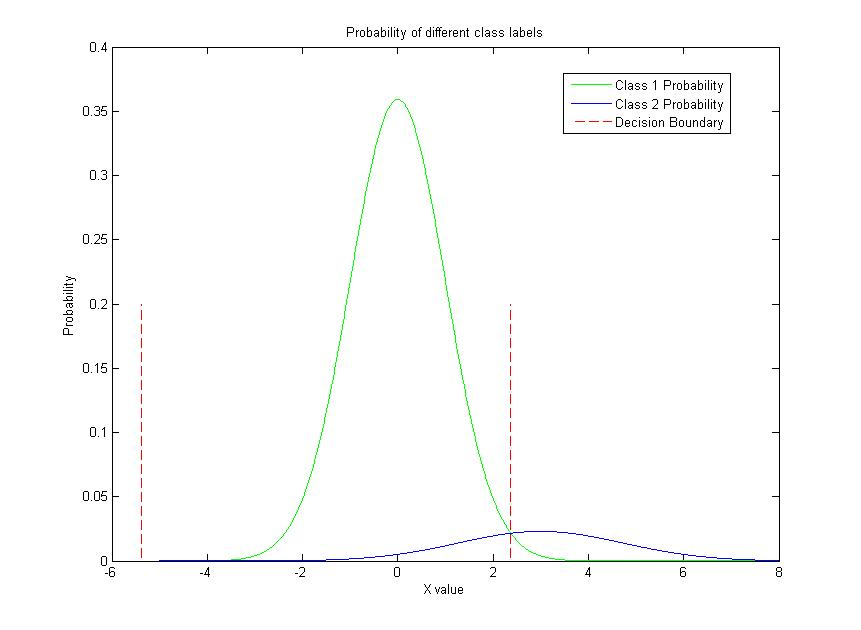
\includegraphics[height=5in]{prob1part2plot.jpg}
\caption{Probability of Class Labels with decision boundaries marked}
\end{figure}

For this case, if we let a and b be the decision boundaries and E be the error, then
\[
E = \int_{-\infty}^{a}{p(c_1|x)p(x) \, dx} + \int_{a}^{b}{p(c_2|x)p(x) \, dx} + \int_{a}^{\infty}{p(c_1|x)p(x) \, dx}
\]
For our case we can simplify this to
\[
E = \int_{-\infty}^{a}{p(x|c_1)p(c_1) \, dx} + \int_{a}^{b}{p(x|c_2)p(c_2) \, dx} + \int_{a}^{\infty}{p(x|c_1)p(c_1) \, dx}
\]
\[
E = 0.9\int_{-\infty}^{a}{p(x|c_1) \, dx} + 0.1\int_{a}^{b}{p(x|c_2) \, dx} + 0.9\int_{a}^{\infty}{p(x|c_1) \, dx}
\]
For this case, according to the Matlab computation, we have $a=-5.3716$ and $b=2.3716$. \\
According to Wolfram Alpha
\[
\int_{-\infty}^{a}{p(x|c_1) \, dx} = \frac{1}{\sqrt{2\pi}} \int_{-\infty}^{-5.3716}{e^{-x^2/2} \, dx} = \frac{9.781 \cdot 10^{-8}}{\sqrt{2\pi}} = 3.90205 \cdot 10^{-8}
\]
\[
\int_{a}^{b}{p(x|c_2) \, dx} = \frac{1}{\sqrt{6\pi}} \int_{-5.3716}^{2.3716}{e^{-(x-3)^2/6} \, dx} = \frac{1.55592}{\sqrt{6\pi}} = 0.358374
\]
\[
\int_{b}^{\infty}{p(x|c_1) \, dx} = \frac{1}{\sqrt{2\pi}} \int_{2.3716}^{\infty}{e^{-x^2/2} \, dx} = \frac{0.0221978}{\sqrt{2\pi}} = 0.00885564
\]
Summing these three together we get the following estimate
\[
E = 0.0438
\]
		
\subsection*{Solution to Problem 2, Part 1}

From previous problem we have to solve
\[
\frac{p(x|c_2)}{p(x|c_1)} \leq \frac{p(c_1)}{p(c_2)}
\]
Given our values we have
\[
\frac{p(x|c_2)}{p(x|c_1)} \leq 1
\]
\[
p(x|c_2) \leq p(x|c_1)
\]
That is when it is optimal to choose $c_1$. This occurs when
\[
exp(-x) \leq 0.5
\]
\[
x \geq log(2)
\]
However, we can only choose $c_1$ for $2 \leq x \leq 4$. Our condition is satisfied in that region, thus the decision regions are as follows:

$c_1$ if $2 \leq x \leq 4$

$c_2$ otherwise

\subsection*{Solution to Problem 2, Part 2}

After putting this all into Matlab, we end up with the following plot
\begin{figure}[H]
\centering
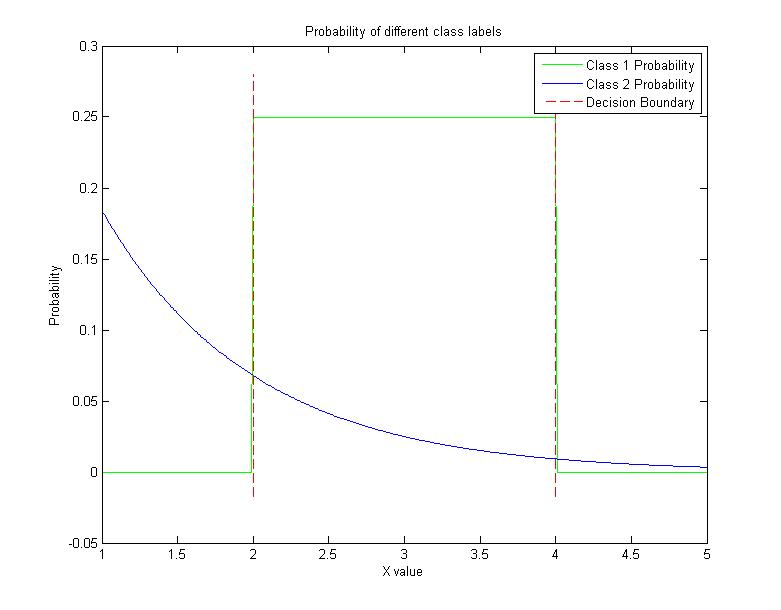
\includegraphics[height=5in]{prob2plot.jpg}
\caption{Probability of Class Labels with decision boundaries marked}
\end{figure}

\subsection*{Solution to Problem 2, Part 3}

For this case, if we let a and b be the decision boundaries and E be the error, then
\[
E = \int_{-\infty}^{a}{p(c_1|x)p(x) \, dx} + \int_{a}^{b}{p(c_2|x)p(x) \, dx} + \int_{a}^{\infty}{p(c_1|x)p(x) \, dx}
\]
For our case we can simplify this to
\[
E = \int_{-\infty}^{a}{p(x|c_1)p(c_1) \, dx} + \int_{a}^{b}{p(x|c_2)p(c_2) \, dx} + \int_{a}^{\infty}{p(x|c_1)p(c_1) \, dx}
\]
\[
E = 0.5\int_{-\infty}^{a}{p(x|c_1) \, dx} + 0.5\int_{a}^{b}{p(x|c_2) \, dx} + 0.5\int_{a}^{\infty}{p(x|c_1) \, dx}
\]
For this case we have $a=2$ and $b=4$. \\
\[
\int_{-\infty}^{a}{p(x|c_1) \, dx} = 0
\]
\[
\int_{a}^{b}{p(x|c_2) \, dx} = \int_{2}^{4}{e^{-x} \, dx} = e^{-2} - e^{-4} = 0.1170
\]
\[
\int_{b}^{\infty}{p(x|c_1) \, dx} = 0
\]
Summing these three together we get the following estimate
\[
E = 0.0585
\]

\subsection*{Solution to Problem 2, Part 4}

From previous problem we have to solve
\[
\frac{p(x|c_2)}{p(x|c_1)} \leq \frac{p(c_1)}{p(c_2)}
\]
Given our values we have
\[
\frac{p(x|c_2)}{p(x|c_1)} \leq 1
\]
\[
p(x|c_2) \leq p(x|c_1)
\]
That is when it is optimal to choose $c_1$. This occurs when
\[
exp(-x) \leq 0.05
\]
\[
x \geq log(20) = 2.9957
\]
However, we can only choose $c_1$ for $2 \leq x \leq 22$. 

$c_2$ if $x \leq log(20)$

$c_1$ if $log(20) \leq x \leq 22$

$c_2$ if $x \geq 22$

After putting this all into Matlab, we end up with the following plot
\begin{figure}[H]
\centering
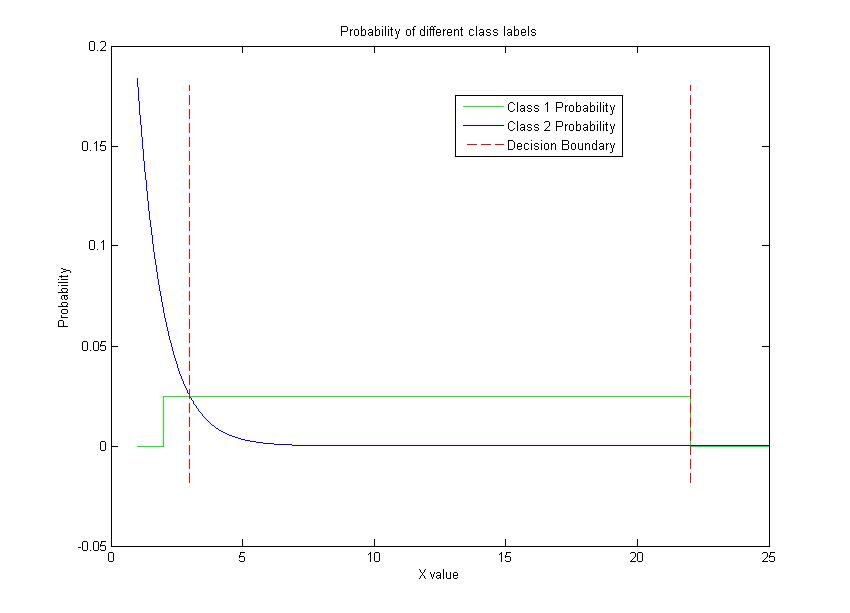
\includegraphics[height=5in]{prob2part2plot.jpg}
\caption{Probability of Class Labels with decision boundaries marked}
\end{figure}

For this case, if we let a and b be the decision boundaries and E be the error, then
\[
E = \int_{-\infty}^{a}{p(c_1|x)p(x) \, dx} + \int_{a}^{b}{p(c_2|x)p(x) \, dx} + \int_{a}^{\infty}{p(c_1|x)p(x) \, dx}
\]
For our case we can simplify this to
\[
E = \int_{-\infty}^{a}{p(x|c_1)p(c_1) \, dx} + \int_{a}^{b}{p(x|c_2)p(c_2) \, dx} + \int_{a}^{\infty}{p(x|c_1)p(c_1) \, dx}
\]
\[
E = 0.5\int_{-\infty}^{a}{p(x|c_1) \, dx} + 0.5\int_{a}^{b}{p(x|c_2) \, dx} + 0.5\int_{a}^{\infty}{p(x|c_1) \, dx}
\]
For this case we have $a=log(20)$ and $b=22$. \\
\[
\int_{-\infty}^{a}{p(x|c_1) \, dx} = \int_{2}^{log(20)}{0.05 \, dx} = (0.05)(log(20)-2) = 0.0498
\]
\[
\int_{a}^{b}{p(x|c_2) \, dx} = \int_{log(20)}^{22}{e^{-x} \, dx} = \frac{1}{20} - e^{-22} = 0.0500
\]
\[
\int_{b}^{\infty}{p(x|c_1) \, dx} = 0
\]
Summing these three together we get the following estimate
\[
E = 0.0499
\]

\subsection*{Solution to Problem 3, Part 1}
First, we will let
\[
K = \frac{1}{(2\pi)^{d/2}|\Sigma|^{1/2}}
\]
\[
f_1(x) = (x-\mu_1)^T \Sigma^{-1} (x-\mu_1)
\]
\[
f_2(x) = (x-\mu_2)^T \Sigma^{-1} (x-\mu_2)
\]
then it holds that
\[
g_1(x) = log(K) - \frac{1}{2}f_1(x) + log(p(c_1))
\]
\[
g_1(x) = -log((2\pi)^{d/2} |\Sigma|^{1/2}) - \frac{1}{2}f_1(x) + log(p(c_1))
\]
\[
g_1(x) = -\frac{1}{2}( d \cdot log(2\pi) + log(|\Sigma|) + f_1(x)) + log(p(c_1))
\]
By the same token
\[
g_2(x) = -\frac{1}{2}( d \cdot log(2\pi) + log(|\Sigma|) + f_2(x)) + log(p(c_2))
\]

\subsection*{Solution to Problem 3, Part 2}

By some algebraic manipulation, it holds that
\[
g(x) = g_1(x)-g_2(x) = - \frac{1}{2} f_1(x) + \frac{1}{2} f_2(x) + log(p(c_1)) - log(p(c_2))
\]
\[
g(x) = \frac{1}{2} ( f_2(x) - f_1(x) ) + log(p(c_1)) - log(p(c_2))
\]
Let $v = 2( log(p(c_2)) - log(p(c_1)) )$ then we have to solve
\[
v = f_2(x) - f_1(x)
\]
\[
(x^T \Sigma - \mu_2^T \Sigma^{-1})(x - \mu_2) - (x^T \Sigma^{-1} - \mu_1^T \Sigma^{-1})(x - \mu_1) = v
\]
\[
(x^T \Sigma^{-1} x - \mu_2^T \Sigma^{-1} x - x^T \Sigma^{-1} \mu_2 + \mu_2^T \Sigma^{-1} \mu_2) - (x^T \Sigma^{-1} x - \mu_1^T \Sigma^{-1} x - x^T \Sigma^{-1} \mu_1 + \mu_1^T \Sigma^{-1} \mu_1) = v
\]
Collecting terms we end up with
\[
(\mu_1^T \Sigma^{-1} - \mu_2^T \Sigma^{-1}) x + x^T (\Sigma^{-1} \mu_1 - \Sigma^{-1} \mu_2) + \mu_2^T \Sigma^{-1} \mu_2 - \mu_1^T \Sigma^{-1} \mu_1 = v
\]
If we let
\[
u = v - \mu_2^T \Sigma^{-1} \mu_2 + \mu_1^T \Sigma^{-1} \mu_1
\]
Then after some factoring we have
\[
(\mu_1^T - \mu_2^T) \Sigma^{-1} x + x^T \Sigma^{-1} (\mu_1 - \mu_2) = u
\]
If we let $\mu_0 = \mu_1 - \mu_2$ then we further have
\[
\mu_0 \Sigma^{-1} x + x^T \Sigma^{-1} \mu_0 = u
\]
If we let $m = \mu_0^T \Sigma^{-1}$ then because $\Sigma^{-1}$ is symmetric, $m^T = \Sigma^{-1} \mu_0$. We thus have
\[
m x + x^T m^T - u = 0
\]
This is the same as
\[
dot(m,x) + dot(m,x) - u = 0
\]
Thus we can further day that
\[
2mx - u = 0
\]
Thus finally let
\[
w = 2m
\]
\[
w_0 = -u
\]
then we have the linear decision boundary

\subsection*{Solution to Problem 3, Part 3}

If $p(c_1) = p(c_2)$ then $v=0$ above, so we have
\[
f_1(x) = f_2(x)
\]
\[
(x-\mu_1)^T \Sigma^{-1} (x-\mu_1) = (x-\mu_2)^T \Sigma^{-1} (x-\mu_2)
\]
The decision boundary is thus when the two MH distances are equal so the class will end up taking on the value of whichever mean is closer. 

\subsection*{Solution to Problem 4, Part 1}

Using problem 3, but where $v=0$, we will use the following variables to simplify our problem
\[
u = \mu_1^T \Sigma^{-1} \mu_1 - \mu_2^T \Sigma^{-1} \mu_2 
\]
\[
\mu_0 = \mu_1 - \mu_2
\]
\[
m = \mu_0^T \Sigma^{-1}
\]
For our purposes, we have $\mu_1=(1,1)$ and $\mu_2=(4,4)$, thus $\mu_0=(-3,-3)$. Additionally
\[
\Sigma^{-1} = \frac{1}{3} \left( \begin{array}{ccc}
4 & -1 \\
-1 & 1 \end{array} \right)
\]
After computing these out, we get the following numbers
\[
u = -15
\]
\[
m = (-3,0)
\]
This leads us to the following numbers for the line
\[
w = (-6, 0)
\]
\[
w_0 = 15
\]
This leads us to the following linear equation
\[
-6 x_1 + 15 = 0
\]
\[
x_1 = 2.5
\]

\begin{figure}[H]
\centering
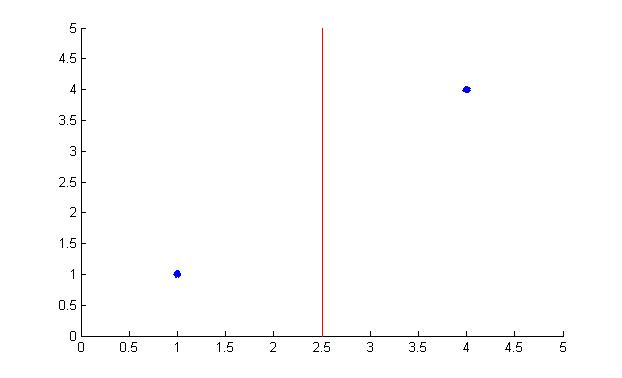
\includegraphics[height=3.25in]{plot4_part1.jpg}
\caption{The decision boundary with the means}
\end{figure}

\subsection*{Solution to Problem 4, Part 2}

The vector for $w$ will be the same as Part 1. The vector for $u$ will be different. We have already found that $u=-15$ when $v=0$, thus for our case, $u = v-15$ so we just need to calculate $v$. By Problem 3, 
\[
v = 2(log(p(c_2)) - log(p(c_1)))
\]
Thus plugging in our values
\[
v = 2( log(0.2) - log(0.8) )
\]
\[
v = 2 ( log(\frac{1}{5}) - log(\frac{4}{5}) )
\]
\[
v = 2 ( -log(5) - ( log(4) - log(5) ) )
\]
\[
v = -2 log(4)
\]
This means that $u = -2log(4)-15$ and thus of course $w_0 = 15+2log(4)$. Our equation for the decision boundary will then become
\[
-6 x_1 + 15 + 2log(4) = 0
\]
\[
x_1 = \frac{15+2log(4)}{6} \approx 2.9621
\]
Because class 1 is weighted higher in this case, its decision region will be bigger, thus the decision boundary will shift toward the mean for class 2, as shown in the below graph. 

\begin{figure}[H]
\centering
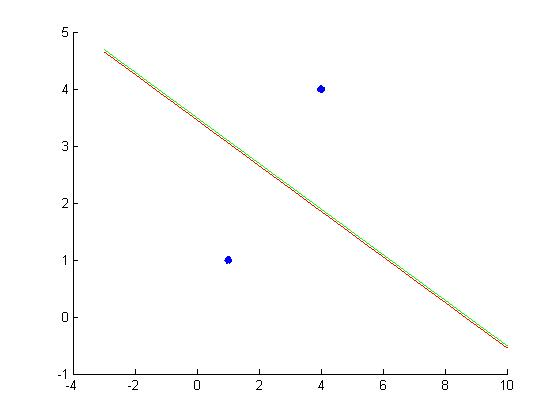
\includegraphics[height=3.25in]{plot4_part2.jpg}
\caption{The decision boundary with the means}
\end{figure}

\subsection*{Solution to Problem 5}

First, you would figure out a probability on the class labels given the parameters of the model, so you need
$p(c|\hat{\theta})$ and $p(c|\hat{\phi})$. You would also attach a prior to the parameters if desired, so you would want $p(\hat{\theta})$ and $p(\hat{\phi})$. 
To figure out the class probability we will say that
\[
p(c|x) = \frac{p(x|c)p(c)}{p(x)}
\]
We can treat $p(x)$ as a normalization constant, thus
\[
p(c|x) \propto p(x|c)p(c)
\]
By law of total probability and adding in the parameters of the model, we can further say that
\[
p(c|x) \propto p(x|c,\hat{\theta})p(c,\hat{\theta}) + p(x|c,\hat{\phi})p(c,\hat{\phi})
\]
\[
p(c|x) \propto p(x|c,\hat{\theta})p(c|\hat{\theta})p(\hat{\theta}) + p(x|c,\hat{\phi})p(c|\hat{\phi})p(\hat{\phi})
\]
Do this for both classes and see which one yields a greater probability. 

\subsection*{Solution to Problem 6}

For this problem, we are assuming that at each pair of points, there is a Gaussian distribution for $y$ given $x$ where the mean $\mu_y = ax+b$ and the variance is $\sigma^2$.
\\
We will define $\theta=(a,b,\sigma)$, then
\[
L(D|\theta) = \prod_{i=1}^N{ \frac{1}{\sigma \sqrt{2\pi}} exp(-\frac{(y_i - (ax_i + b))^2}{2\sigma^2})}
\]
Taking the log to get log-likelihood we have
\[
l(\theta) = -\frac{N}{2} log(2\pi \sigma^2) + \sum_{i=1}^N{-\frac{(y_i - (ax_i + b))^2}{2\sigma^2}}
\]
Simplifying further we have
\[
l(\theta) = -\frac{N}{2} log(2\pi \sigma^2) - \frac{1}{2\sigma^2} \sum_{i=1}^N{(y_i - (ax_i + b))^2}
\]
Expanding out the square we have
\[
l(\theta) = -\frac{N}{2} log(2\pi \sigma^2) - \frac{1}{2\sigma^2} \sum_{i=1}^N{y_i^2 -2y_i (ax_i + b) + (ax_i + b)^2}
\]
Expanding out the square again
\[
l(\theta) = -\frac{N}{2} log(2\pi \sigma^2) - \frac{1}{2\sigma^2} \sum_{i=1}^N{[y_i^2 -2ay_i x_i -2by_i + a^2 x_i^2 + 2abx_i + b^2]}
\]
We will find $\hat{a}_{ML}$ and $\hat{b}_{ML}$ by first taking the partials
\[
\frac{\partial l}{\partial a} = - \frac{1}{2\sigma^2} \sum_{i=1}^N{[-2y_i x_i + 2a x_i^2 + 2bx_i]}
\]
\[
\frac{\partial l}{\partial b} = - \frac{1}{2\sigma^2} \sum_{i=1}^N{[-2y_i + 2a x_i + 2b]}
\]
Setting both equal to zero we end up having to solve the following equations
\[
\sum_{i=1}^N{[-y_i x_i + a x_i^2 + bx_i]} = 0
\]
\[
\sum_{i=1}^N{[-y_i + a x_i + b]} = 0
\]
Rearranging the sums and putting into a linear system form, we have the solve the following
\[
a\sum_{i=1}^N{x_i^2} + b\sum_{i=1}^N{x_i} = \sum_{i=1}^N{y_i x_i}
\]
\[
a\sum_{i=1}^N{x_i} + b \cdot N = \sum_{i=1}^N{y_i}
\]
For shorthand, we will now let
\[
A = \sum_{i=1}^N{x_i^2}
\]
\[
B = \sum_{i=1}^N{x_i}
\]
\[
C = \sum_{i=1}^N{y_i x_i}
\]
\[
D = \sum_{i=1}^N{y_i}
\]
Then we are left with solving
\[ \left( \begin{array}{ccc}
A & B \\
B & N \end{array} \right)
\left( \begin{array}{ccc}
a \\
b \end{array} \right)=
\left( \begin{array}{ccc}
C \\
D \end{array} \right)\]
After doing the matrix inverse, we have the following 
\[ 
\left( \begin{array}{ccc}
a \\
b \end{array} \right) =
\frac{1}{AN - B^2}
\left( \begin{array}{ccc}
N & -B \\
-B & A \end{array} \right)
\left( \begin{array}{ccc}
C \\
D \end{array} \right)
\]
Thus finally we can say that
\[
\hat{a}_{ML} = \frac{NC-BD}{AN-B^2}
\]
\[
\hat{b}_{ML} = \frac{AD-BC}{AN-B^2}
\]
We now want to find $\hat{\sigma^2}_{ML}$. If we let
\[
K = \sum_{i=1}^N{(y_i - (ax_i + b))^2}
\]
then we will have after letting $v = \sigma^2$
\[
l(\theta) = -\frac{N}{2} log(2\pi v) - \frac{K}{2v}
\]
Taking the derivative with respect to v we have
\[
l'(\theta) = -\frac{N}{2v} + \frac{K}{2v^2}
\]
Setting it equal to zero we have to solve
\[
Kv = N v^2
\]
We can assume a non-zero variance so we can assert that
\[
v = \frac{K}{N}
\]
Finally we can say that
\[
\hat{\sigma^2}_{ML} = \frac{1}{N} \sum_{i=1}^N{(y_i - (\hat{a}_{ML}x_i + \hat{b}_{ML}))^2}
\]
\end{document}








